% UGA Dissertation Template
% Changes to official template by Kyle Krafka (December 2015)

\documentclass[12pt,notitlepage]{report}  % The notitlepage option prevents \maketitle from resetting page numbering, below.
\usepackage{kyle}
\usepackage{fullpage}
\usepackage{listings}
\usepackage{setspace}\doublespacing
\textfloatsep 0.75in
\usepackage[nottoc]{tocbibind}  % Added nottoc option to remove "Contents"
\usepackage{graphicx}
\usepackage{subcaption}
\usepackage{wrapfig}
\usepackage[hidelinks]{hyperref}  % Allows you to click on references in the PDF.
\usepackage[square]{natbib}  % Use name/year for citations rather than numbers.
\usepackage{amsmath}
% \usepackage{MinionPro}  % Serif font.
% \usepackage{MyriadPro}  % Sans-serif font.
\usepackage{pgfornament}  % For the ornament, used on the dedication page.
\newtheorem{hyp}{Hypothesis}
\usepackage{multirow}
\usepackage{color}
\usepackage{url}
\renewcommand{\lstlistingname}{Snippet}
\renewcommand\lstlistlistingname{List of Code Snippet}
% \usepackage{longtable}
% This makes for a larger left margin so that when you bind your dissertation,
% the text stays away from the binding. From what I have seen, people typically
% have it bound single-sided (i.e., the back of each page is blank), but if you
% want it double-sided, use the "twoside" option right before or after the
% "bindingoffset" option here (with a comma). The choice of 6 mm was mostly
% arbitrary, but The Graduate School recommended anywhere from 0 to 0.5 inches
% of binding offset on top of the 1 in left margin.
\usepackage[bindingoffset=6mm]{geometry}
\usepackage[toc]{appendix}  % Allows for an appendix, which should appear in the table of contents.
\usepackage[english]{babel}
\usepackage{lipsum}  % Generates dummy text
\definecolor{dkgreen}{rgb}{0,0.6,0}
\definecolor{gray}{rgb}{0.5,0.5,0.5}
\definecolor{mauve}{rgb}{0.58,0,0.82}

\lstset{ %
    columns=fixed,
    % basicstyle=\footnotesize\ttfamily,
    numbers=left,                                        % 在左侧显示行号
    frame=none,                                          % 不显示背景边框
    backgroundcolor=\color[RGB]{245,245,244},            % 设定背景颜色
    keywordstyle=\color[RGB]{40,40,255},                 % 设定关键字颜色
    numberstyle=\footnotesize,           % 设定行号格式
    commentstyle=\it\color[RGB]{0,96,96},                % 设置代码注释的格式
    stringstyle=\rmfamily\slshape\color[RGB]{128,0,0},   % 设置字符串格式
    showstringspaces=false,                              % 不显示字符串中的空格
    language=C++,                                        % 设置语言
    xleftmargin=2em,
    xrightmargin=2em,
    aboveskip=2em,
    belowskip=2em,
    upquote=true,
    literate = {-}{-}1,
}

% Title
\newcommand{\dissertationtitle}{STANDALONE CONSTRAINT SOLVER FOR ASYNCHRONOUS SYMBOLICEXECUTION}
\newcommand{\whoami}{Jiakuan Li}

\setcounter{tocdepth}{1}

\begin{document}

% Make the official abstract page
\newpage
\thispagestyle{empty}
\vspace*{18pt}
\begin{center}
\textsc{\large{\dissertationtitle}}\\[18pt]  % A little larger than the original template
by\\[18pt]
\textsc{\whoami}\\[12pt]
(Under the Direction of Kang Li)\\[12pt]
\textsc{Abstract}
\end{center}
Symbolic execution is a technique to analyze a binary. It symbolizes the input of a program and try to generate testcases that covered all of the feasible path. The constraint solver is one of the indispensable and the most critical components in a symbolic execution engine. All of the symbolic execution engines rely on solvers to conduct testcases and guide the exploration during the operation process. Currently, and engine regularly spends comparatively long time solving the constraints. To shorten the time for analyzing a binary, using a standalone solver is one of the practical strategies. In my research, I implemented a standalone solver that takes in kquery strings and generating testcases according to the constraints in that kquery it receives. Moreover, to improve the performance of the solver, the solver now can share caches.
\thispagestyle{empty}

\begin{list}{\textsc{Index words:\hfill}}{\labelwidth 1.2in\leftmargin 1.4in\labelsep 0.2in}
\item 
\begin{flushleft}\singlespacing
KLEE,
Symbolic Execution,
Constraint Solver
\end{flushleft}
\end{list}

% Make the official title page
\newpage
\pagenumbering{roman}
\thispagestyle{empty}
\vspace*{18pt}
\begin{center}
\textsc{\large{\dissertationtitle}}\\[18pt]
by\\[18pt]
\textsc{\whoami}\\[12pt]
B.S., University of Georgia, 2016\\
\vfill
A Dissertation Submitted to the Graduate Faculty \\
of The University of Georgia in Partial Fulfillment \\
of the \\
Requirements for the Degree \\[10pt]
\textsc{Master of Science}\\[36pt]
\textsc{Athens, Georgia}\\[18pt]
2018
\end{center}

% Make the copyright page
\newpage
\thispagestyle{empty}
\vspace*{5.5in}
\begin{center}
\copyright 2018 \\
\whoami \\
All Rights Reserved
\end{center}

% Make the approval page
\newpage
\thispagestyle{empty}
\vspace*{18pt}
\begin{center}
\textsc{\large{\dissertationtitle}}\\[18pt]
by\\[18pt]
\textsc{\whoami}
\end{center}
\vfill
\begin{flushleft}\singlespacing
\hskip 200pt {Approved:}\\
\vskip 12pt

% If you have two major professors, change "Professor" to "Professors."
\hspace*{200pt}\makebox[100pt][l]{Major Professor:}Kang Li\\
\vskip 12pt
% Committee (use as many lines as needed)
\hspace*{200pt}\makebox[100pt][l]{Committee:       }Kyu H. Lee\\
\hspace*{200pt}\makebox[100pt][l]{~                }Maria Hybinette\\
% Approval words
\vfill
Electronic Version Approved:\\[12pt]
Suzanne Barbour\\
Dean of the Graduate School\\
The University of Georgia\\
August 2018
\end{flushleft}

% This title page is not in the style manual, but it is in the original template.
\title{\textbf{\dissertationtitle}}
\author{\whoami}
\date{August 2018}
\maketitle
\thispagestyle{empty}

\newpage
\vspace*{1.5in}
\begin{center}
\emph{For My Parents}\\
\vspace{1cm}
\pgfornament[width = 4cm,
             color = black]{88}  % Feel free to download the pgfornament manual to choose your own ornament.
\end{center}

\chapter*{Acknowledgments}
% chapter* removes chapter number, but also removes from TOC, so we add it back
\addcontentsline{toc}{chapter}{Acknowledgments}

I would like to thank my thesis advisor Professor Kang Li at The University of Georgia. Professor Li always answered my questions patiently whenever I ran into trouble of my research or had problems of implementing the projects. He consistently allowed this thesis to be my own work but steered me it in the right direction. More important, I learned a lot of research skills as well as presenting skills from him. I am sure that these skills will benefit me in my future career.

I would also like to thank my colleagues in Network System and Security Lab. Working with such a great team will always be my pleasure. We worked together to solve engineering problems also discussed our research together, which are mind refreshing and incredibly inspiring for me and even this thesis. 

Finally, I must express my very profound gratitude to my girlfriend Yunying Xu for providing me with unfailing support and continuous encouragement throughout my years of study and through the process of researching and writing this thesis. This accomplishment would not have been possible without her.

I hope this thesis will not be my final destination of academic research, and hope it is not just a hope.

\tableofcontents
\listoffigures  % If any.
\listoftables % If any.
\lstlistoflistings
\clearpage
\pagenumbering{arabic}

% Chapters. Organize and name as you wish, as long as these refer to files that exist.
%%%%%%%%%%%%%%%%
% INTRODUCTION %
%%%%%%%%%%%%%%%%
\chapter{INTRODUCTION}% Chapter titles are capitalized -- UNLV rule.

Symbolic Execution \cite{King:1976:SEP:360248.360252} is a technique that can explore all of the possible paths of a binary using a constraint solver. The method came out a long time ago, but until recentdays \cite{symbolic-execution}, it has gathered significant attention. People implemented several tools and found bugs and security vulnerabilities that buried very deep in the code in different software applications \cite{sybolic-execution-in-practice}.

The reason of why symbolic execution gathered significant attention in the recent few years is because of the development of the SMT solver \cite{DeMoura:2011:SMT:1995376.1995394}. But still, constraints solver remains one of the main challenges of symbolic execution \cite{multi-solver-support}. As a result, to increase the speed of a symbolic execution engine, we can either improve the solving speed of the solver or optimize how the symbolic execution uses the engine. Moreover, let the solver uses previous constraint result is another option. 

\section{Problem Statement}
All of the current symbolic execution engines can systematically cover all the feasible path for a binary during its analysis process. However, it has its disadvantages, that is symbolic execution engine are slower than another type of dynamic analysis tools. So, can we use some other techniques to help the analysis process go faster? I target my research on one of the popular symbolic execution tool, KLEE \cite{Cadar:2008:KUA:1855741.1855756}, and try to shorten the analysis time for a program.

\section{Research Method}

The symbolic execution engine KLEE is a synchronous engine. During its execution, it is always waiting for the response from the solver to continue the exploration. While asking the solver to generate testcases, that means the current path reaches the end, and the rest of the path exploration does not rely on that result. Therefore, waiting for the solver's response is wasting time. 

    \begin{hyp}
    \textit{Making a KLEE in asynchronous mode can significantly reduce the time that is required for covered all the path in a program.}
    \end{hyp}
    
In addition to providing KLEE an asynchronous mode, solver optimization is one of the research's goal. KLEE's implementation allows the solver using cache, so let the standalone solver using cache is one of the optimization methods.

    \begin{hyp}
    \textit{Allowing the standalone solver using cache can reduce the number of counterexamples that generated by the solver.}
    \end{hyp}

\section{Contribution}

In this research, I have the following contributions:
\begin{itemize}
    \item Allow KLEE to analysis the program in asynchronous mode.
    \item Adding feature of produce testcases for every branch node that has a possible path.
    \item Implementing a server to receive query command that KLEE sends out during the analysis process.
    \item Wrapping up a solver that checks the cache for the query before throwing it into the SMT solver to generate a counterexample. 
\end{itemize}
\section{Outline}
This thesis is consist of the following chapters.
\begin{itemize}
    \item Chapter 2: Background Knowledge and Related Work
    \item Chapter 3: Implementation
    \item Chapter 4: Experimental Evaluation
    \item Chapter 5: Summary and Conclusion
\end{itemize}
\chapter{BACKGROUND KNOWLEDGE AND RELATED WORK}
In this chapter, I will introduce the background knowledge of symbolic execution and the related work of my research.
\section{What is Symbolic Execution?}

Symbolic Execution is one of the program analysis techniques whose ultimate goal is to systematically cover all the feasible paths by solving the paths' constraints by using an SMT (Satisfiability Modulo Theory). In order to get the idea of what symbolic execution really is, I will use Snippet \ref{simple_program} as an example to explain the detail of symbolic execution.
\pagebreak
\begin{spacing}{1}
{
\begin{lstlisting}[frame=shadowbox, caption={A Simple Program},label={simple_program}]
int x = 0, y = 0, z = 0;
if (a) {
    x = -2;
}
if (b < 5) {
    if (!a && c) {
        y = 1;
    }
    z = 2;
}
assert(x+y+z != 3)
\end{lstlisting}
}
\end{spacing}

In static analysis, the value of \texttt{x}, \texttt{y} and \texttt{z} will be assigned a variable, then walk through the program to see what part of the code is covered. Then reassign values to \texttt{x}, \texttt{y}, and \texttt{z} and repeat this step until all the possible paths are covered. Apparently, this method is a very low-efficiency method because there is no guarantee that every execution will have a new path be covered. 

Unlike static analysis, symbolic execution is way more efficient. In symbolic execution, no values will be assigned to \texttt{x}, \texttt{y}, and \texttt{z}. Instead, the variables \texttt{x}, \texttt{y}, and \texttt{z} are treated as ``symbol.'' When the execution hit line 2, two constraints will be added. They are \texttt{a == 1} and \texttt{a != 1} representing the \texttt{true} and \texttt{false} of the if-statement respectively. These constraints will be added to two buckets. Each bucket is representing a possible path of this program. Then the engine will continue executing. Once it hits line 5, like the if-statement in line2, two constraints will be produced and added to the buckets. And finally, connecting all the constraints in each bucket with the \texttt{AND} logical operator, an assignment for that path is generated.

\begin{figure}[h]%This [h] tells LaTeX to try to put the picture here.
                 %Without it, it will go to the top of the next page.
\begin{center}
{\mbox{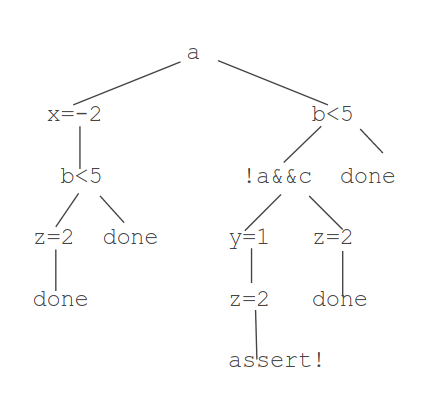
\includegraphics[height=200pt]{figures/path_tree.png}}}
\end{center}
\caption{\label{path_tree}Path Conditions}
\end{figure}

Figure \ref{path_tree} is a tree of path condition of the Snippet \ref{simple_program}. Each of the nodes is a line of code. If a tree node has two children, it means the there is a possible path at that node. Also, the left child representing the \texttt{true} path and the right child representing the \texttt{false} path. To activate the left most path, the testcase should fulfill the constraints of \texttt{(a == 1 AND b < 5)}. To activate the second from the left path, the testcase should fulfill the constraints of \texttt{(a == 1 AND b >= 5)}. To assert, the constraints is \texttt{(a != 1 AND b < 5 AND c == 1)}. The constrains for the rest of two paths is \texttt{(a != 1 AND b < 5 AND c != 1)} and \texttt{(a != 1 AND b >= 5)} respectively.

Comparing static analysis and symbolic execution, the main difference is that symbolic execution get the assignment according to the path it explored, and static analysis gets the assignment before exploring the path. As we can see, there are five possible paths in the program. Therefore, five testcases will be generated to cover all the paths after the symbolic execution process. But for static analysis, probably more than five testcases will be generated to cover all of the feasible paths.

\section{KLEE}

\begin{figure}[h]
\begin{center}
{\mbox{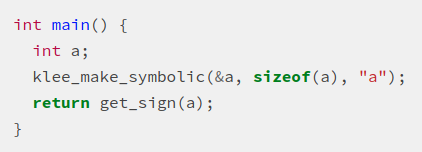
\includegraphics[height=100pt]{figures/make_symbolic.png}}}    
\end{center}
\caption{\label{make_symbolic}Make Input As Symbolic}
\end{figure}

KLEE is a symbolic execution tool that can generate testcases that achieve high coverage on a variety of complex and environmentally-intensive programs automatically \cite{Cadar:2008:KUA:1855741.1855756}. Using the GNU \texttt{COREUTILS} as a benchmark, they covered 90\% of the code on average for all 89 utilities in the package. KLEE can only test the programs that are written in C/C++ and have the source code available. First, a function \texttt{klee\_make\_symbolic} need to be added to the code to mark the input as symbol. Figure \ref{make_symbolic} demonstrates how to make the input symbolic. Then compile the code into LLVM bytecode. The reason for doing so is because KLEE simulates the system environment to handle environmentally-intensive programs. KLEE will execute every line of bytecode to maintain the stack, heap, and etc. for the environment. 

To understand how KLEE works, a critical structure that KLEE implemented need to be introduced. It is \texttt{ExecutionState}. Snippet \ref{execution_state} shows the detail of \texttt{ExecutionState}. \texttt{pc} is the pointer to an instruction to be executed after the current instruction, \texttt{prevPC} is the pointer to the instruction which is currently executed, \texttt{stack} representing the current instruction stream, and \texttt{constraints} collects the constraints so far. Each \texttt{ExecutionState} is representing a valid path. KLEE define a set of operations for each of LLVM instructions. Modifying the data in \texttt{ExecutionState} is completed in those operations. Everytime KLEE hit an if-statement/while-loop/switch-statement or any other instructions that can possibly have a new path; it checks the feasibility of the instruction. If the path is feasible, KLEE will make a copy of the current \texttt{ExecutionState}, and added positive constraints and negative constraints to current \texttt{ExecutionState} and the duplicate. KLEE called this operation \texttt{fork}. After the \texttt{fork} operation complete, KLEE will assign new \texttt{pc} to the current \texttt{ExecutionState} and its copy based on their constraints. Then both of the current \texttt{ExecutionState} and its copy will be put back to the pool and waiting for next round of execution.

Talking at a high level, KLEE completes the analysis task in the following manner. 
\begin{enumerate}
    \item Select one \texttt{ExecutionState} from the pool.
    \item Execute the instruction that \texttt{prevPC} pointed to.
    \item Update the \texttt{ExecutionState} pool.
    \item Repeat step 1.
\end{enumerate}
Snippet \ref{main_logic} indicate this logic. \texttt{states} is the pool of \texttt{ExecutionState}, \texttt{searcher} is responsible for selecting state to execute from \texttt{states}. By default, KLEE will randomly select one \texttt{ExecutionState} from the pool, but it can be depth-first search or a breadth-first search as user's preference.

\begin{spacing}{1}
{
\begin{lstlisting}[frame=shadowbox, caption={ExecutionState},label={execution_state}]
class ExecutionState{
...
KInstIterator pc;
KInstIterator prevPC;
stack_ty stack;
...
ConstraintManager constraints;
...
}
\end{lstlisting}
}
\end{spacing}
\clearpage
\begin{spacing}{1}
{
\begin{lstlisting}[frame=shadowbox, caption={KLEE's Main Logic},label={main_logic}]
while (!states.empty() && !haltExecution) {
    ExecutionState &state = searcher->selectState();
    KInstruction *ki = state.pc;
    ...
    executeInstruction(state, ki);
    ...
    updateStates(&state);
}
\end{lstlisting}
}
\end{spacing}
While the \texttt{ExecutionState} reaches the end or \texttt{pc} points to an invalid address, KLEE will generate a  testcase for that \texttt{ExecutionState} using the solver. The solver consumes the \texttt{constraints} of the \texttt{ExecutionState} and generate a testcase. After receiving the testcase from the solver. The \texttt{ExecutionState} object will be deleted.

\section{Solver}

By default, KLEE uses STP \cite{Ganesh:2007:DPB:1770351.1770421} as the internal solver, but Z3 \cite{DeMoura:2008:ZES:1792734.1792766} can be an option. In general, STP solver emerges as a winner over Z3. By benchmarking \text{[}, \texttt{base64}, \texttt{chmod}, \texttt{comm}, \texttt{csplit}, \texttt{dircolors}, \texttt{echo}, \texttt{env}, \texttt{factor}, \texttt{join}, \texttt{ln} and \texttt{mkfifio}, STP consumes 1,713s to complete, and Z3 takes 3609s \cite{multi-solver-support}. Although KLEE has already got a robust solver, they still have a lot of optimization on the solver side to help the solver run faster. KLEE developed two optimization method on the solver side -- Independent Constraint and Cache. Figure \ref{klee_optimization} shows they process of optimization developed by KLEE.

A query is consist of constraints. Among those constraints, some of them are related, and some of them are not. What KLEE does is they separate the query into little pieces. Each of the pieces contains a set of constraints that have no relation with other constraints. Chopping the query into smaller pieces can not only help the solver to obtain the result faster but also benefits the Cache optimization method as well.

Look up cache before throwing the query to the solver one the useful optimization at the solver side. KLEE maintain a \texttt{Map} in the engine. Using the constraint itself as the key and the counterexample that the solver generates as the value. Before asking solver for the counterexample, KLEE will first check if there is a solved one previously. The idea of this method is query \texttt{Map} is in constant time. Since the \texttt{Map} is maintained in the RAM, ideally, the look up speed should be way more faster than asking solver to generate a counterexample especially when the query is very complicate.

\begin{figure}[h]%This [h] tells LaTeX to try to put the picture here.
                 %Without it, it will go to the top of the next page.
\begin{center}
{\mbox{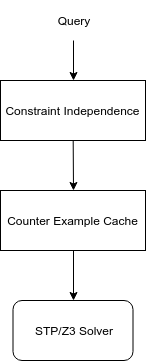
\includegraphics[height=250pt]{figures/klee_optimization.png}}}
\end{center}
\caption{\label{klee_optimization}KLEE's Optimization Method}
\end{figure}

\section{KQuery}

KQuery is a textual representation of the constraint expressions and queries \cite{KQuery}. Currently, KQuery is able to represent a quantifier-free formulas over bitvectors and arrays. It is designed to be easy read and write. Like many other programming languages require variables to be declared before using, bitvectors and arrays need to be declare before querying. A valid query should have the array declaration part and a query command part. Figure \ref{kquery_declaration} shows the syntax of the KQuery declaration. Figure \ref{kquery_query} shows the syntax of a valid query command.

\begin{figure}[h]%This [h] tells LaTeX to try to put the picture here.
                 %Without it, it will go to the top of the next page.
\begin{center}
{\mbox{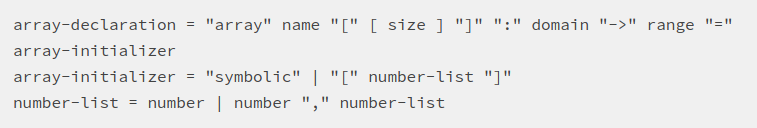
\includegraphics[height=70pt]{figures/kquery_declaration.png}}}
\end{center}
\caption{\label{kquery_declaration}KQuery's Declaration Syntax}
\end{figure}

\begin{figure}[h]%This [h] tells LaTeX to try to put the picture here.
                 %Without it, it will go to the top of the next page.
\begin{center}
{\mbox{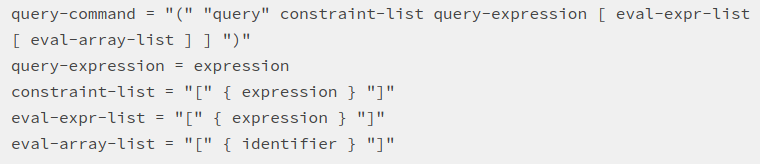
\includegraphics[height=90pt]{figures/query_command.png}}}
\end{center}
\caption{\label{kquery_query}KQuery's Query Command Syntax}
\end{figure}

Combine both the declaration part and the query part can construct a valid query command in the format of KQuery. Snippet \ref{kquery} is a valid query in KQuery format. Translating this query command back to plain English, it is ``Having an array of size 10. The value at the index of 0 is Equal to 77''. For this query command, the solver should return ``\texttt{M000000000}". Note, since the constraint does not have any restriction of other values, the solver will put 0 on those indices by default.

\begin{spacing}{1}
{
\begin{lstlisting}[frame=shadowbox, caption={KQuery},label={kquery}]
array foo[10]: w32 -> w8 = symbolic
(query [(Eq 77 (Read W8 0 foo))] false [] [foo])
\end{lstlisting}
}
\end{spacing}

Not limited to the comparisons, the expression also supports arithmetic operations, bitwise operations. Figure \ref{arithmetic_operations} shows the syntax of arithmetic operations. Figure \ref{bitwise_operations} shows the syntax of bitwise operations. Figure \ref{comparisons} shows the syntax of the comparisons.

\begin{figure}[h]%This [h] tells LaTeX to try to put the picture here.
                 %Without it, it will go to the top of the next page.
\begin{center}
{\mbox{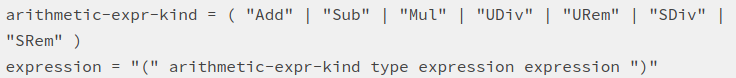
\includegraphics[height=45pt]{figures/arithmetic.png}}}
\end{center}
\caption{\label{arithmetic_operations}KQuery's Arithmetic Operation Syntax}
\end{figure}

\begin{figure}[h]%This [h] tells LaTeX to try to put the picture here.
                 %Without it, it will go to the top of the next page.
\begin{center}
{\mbox{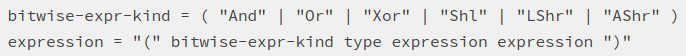
\includegraphics[height=35pt]{figures/bitwise.png}}}
\end{center}
\caption{\label{bitwise_operations}KQuery's Bitwise Operation Syntax}
\end{figure}

\begin{figure}[h]%This [h] tells LaTeX to try to put the picture here.
                 %Without it, it will go to the top of the next page.
\begin{center}
{\mbox{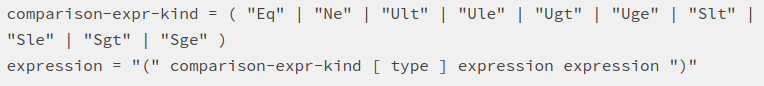
\includegraphics[height=50pt]{figures/comparisons.png}}}
\end{center}
\caption{\label{comparisons}KQuery's Comparisons Syntax}
\end{figure}

The meaning of the expression kinds in arithmetic operations are defined as below:\\
\texttt{Add}: add operation\\
\texttt{Sub}: subtract operation\\
\texttt{Mul}: multiply operation\\
\texttt{UDiv}: truncated unsigned division. Undefined if divisor is 0.\\
\texttt{URem}: Unsigned remainder. Undefined if divisor is 0.\\
\texttt{SDiv}: Signed division. Undefined if divisor is 0.\\
\texttt{SRem}: Signed remainder. Undefined if divisor is 0. Sign of the remainder is the same as that of the dividend.\\

The meaning of the expression kinds in bitwise operations are defined as below:\\
\texttt{And}: and operation.\\
\texttt{Or}: or operation.\\
\texttt{Xor}: xor operation.\\
\texttt{Shl}: logical shift left. For example, \texttt{(Shl TYPE X Y)} means moves each bit of \texttt{X} to the left by \texttt{Y} positions. The \texttt{Y} right-most bits of \texttt{X} are replaced with zero, and the left-most bits discarded.\\
\texttt{LShr}: logical shift right.\\
\texttt{AShr}: arithmetic shift right. Behaves as \texttt{LShr} except that left-most bit of \texttt{X} copy the initial left-most bit of \texttt{X}.\\

The meaning of the expression kinds of comparisons are defined as below:\\
\texttt{Eq}: equal.\\
\texttt{Ne}: not equal.\\
\texttt{Ult}: unsigned less than.\\
\texttt{Ule}: unsigned less or equal to.\\
\texttt{Ugt}: unsigned greater than.\\
\texttt{Uge}: unsigned greater or equal to.\\
\texttt{Slt}: signed less than.\\
\texttt{Sle}: signed less or equal to.\\
\texttt{Sgt}: signed greater than.\\
\texttt{Sge}: signed greater or equal to.\\
\section{Related Work}

The goal of this thesis is to address the the most significant issue of symbolic execution. A lot of people have done some fantasitc work to solve this problem before. I was inspired by one of the previous projects. In that project, the researchers modified KLEE's own data structure to serialize a query in order to send out to the remote solver \cite{Rakadjiev:2015:PSS:2847598.2847727}. This method has fast query transfer speed. However, it limits the symbolic execution engine to be KLEE. It can't support multiple different symbolic execution tools working at the same time. To avoid this disadvantages, I decided to send out a query in KQuery format. Since KQuery is a textual representation of the queries and constraints, technically, all of the constraints can be represented in the format of KQuery. This method allows another engine to use the remote solver by sacrificing some of the query transfer time.

In my remote solver, I also adopt KLEE's optimization method -- Constraint Independence and Caching. The main difference is that KLEE uses cache for the same program because KLEE is a synchronous engine. The solver is built-in in the engine. Once KLEE finishes the analysis task, the solver will be terminated and cache will be cleared. My solver is a remote solver, and it will not be terminated. Therefore, the cache will always exist. All of the queries can share the same cache map. I argue that this method can reduce the number of counterexample that generates by the solver. 
\chapter{IMPLEMENTATION}%Titles must be capitalized.

In this chapter, I will introduce how I modified the KLEE to add an asynchronous mode to it as well as how do I wrapping the solver to use it as a standalone solver. Moreover, a new feature is added to KLEE. It is called ``otherside testcase generation``.

\section{Asynchronous Mode}
As I mentioned in Chapter 2, KLEE is a synchronous symbolic execution tool. KLEE will wait for the result from the solver even though it is not necessary to do so. Figure \ref{klee_control_flow} shows the control flow of KLEE. After terminating an \texttt{ExecutionState}, KLEE will ask solver to solve the constraints in that \texttt{ExecutionState} and wait for the result. Then checking if there is any \texttt{ExecutionState} waiting to be executed in the pool. However, KLEE will not use the result that it waits for. Previous research has pointed out that symbolic execution engine spends 90\% of their time in solver constraints \cite{Rakadjiev:2015:PSS:2847598.2847727}. Therefore, waiting for a result that it will not use anymore is wasting time. Alternatively, the solver can solve the constraints alone. KLEE is not helping the solver while it is waiting for the result. KLEE should keep executing other \texttt{ExecutionState} left in the pool. This improvement can significantly shorten the time for analyzing a program. In other words, the analysis task will finish much earlier than before. And the analyzing time relies on the engine's performance instead of solver's performance. 

\begin{figure}%This [h] tells LaTeX to try to put the picture here.
                 %Without it, it will go to the top of the next page.
\begin{center}
{\mbox{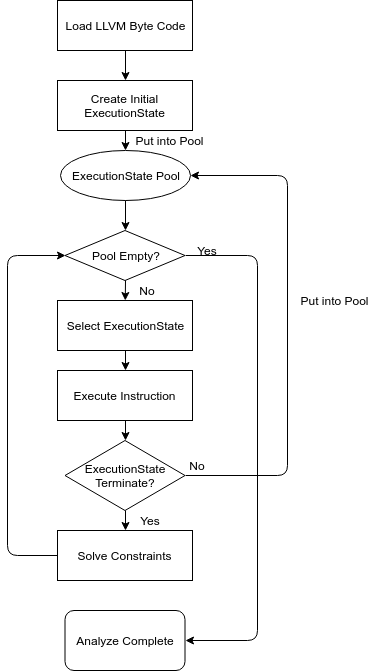
\includegraphics[height=500pt]{figures/klee_control_flow.png}}}
\end{center}
\caption{\label{klee_control_flow}KLEE Original Control Flow}
\end{figure}


To transmit queries, I decided to send out the constraints in the KQuery format using HTTP \texttt{POST} method. The decision is under following consideration. KLEE has its special data structure to represent constraints. If a query needs to be sent out, it requires data serialization. Once the solver receives the query and deserializes it, it turns out to be KLEE's data structure. Under this setting, solver becomes ``KLEE-ONLY'' because the solver does not know about other engine's data structure and unable to handle those queries from other symbolic execution engines. Also, sending queries in KQuery format reduce the work for changing backend solver. All constraints solver has their own interface. Connecting symbolic execution engine's  data structure to different solver's interface requires a solid understanding of data structure from the engine. However, if the solver only receives queries written in KQuery format, we just need to know how to connect KQuery to solver's interface if we need to replace the backend solver, even though the engine changes its own data structure in the future. Moreover, KQquery is a human readable representation. When we need to debug the solver, KQuery can make it easier. Receiving queries in KQuery has such advantages, yet nothing is perfect. Presenting constraints in KQuery needs conversion time, and the process of conversion takes longer than the serialize the data structure of the symbolic engine. At the solver side, parsing the queries in KQuery into the data structure that can be used in solver's interface also takes longer than the data deserialization. After carefully considering the trade-off between speed and scalability, I decided to transfer the query command in KQuery format instead of serializing the original data structure of the symbolic execution tool.

Once deciding how to transmit the queries to the remote solver, the rest of the implementation is straightforward. In KLEE's implementation of terminating an execution path, they first ask the solver to generate a testcase based on the constraints that the tool collected during the execution. Then delete the \texttt{ExecutionState}. In my implementation, I took out the constraints from the \texttt{ExecutionState}, then convert them into the format of KQuery and send it to the remote server via \texttt{HTTP POST} request.

% \begin{figure}[h]%This [h] tells LaTeX to try to put the picture here.
%                  %Without it, it will go to the top of the next page.
% \begin{center}
% {\mbox{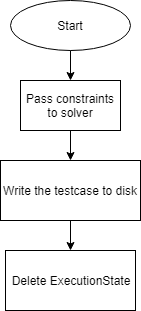
\includegraphics[height=250pt]{img/KLEE_terminate.png}}}
% \end{center}
% \caption{\label{klee_control_flow}KLEE's Workflow Terminating a State}
% \end{figure}

In addition to providing KLEE an asynchronous mode, testcases generation for a concrete input of a program is also provided. Feeding in a concrete input, if the input went through some ``forkable'' statement, then generate the testcase to hit the ``opposite'' branch. For example, Snippet \ref{get_sign} is a program get the sign of an integer, feeding a concrete input ``1'', the program will return ``positive''. In this case, the ``opposite'' branches are the return of ``negative'' and ``Zero.'' So feeding in a concrete input ``1'', the testcases generation for that concrete input will generate two testcases that contains a negative number and contains a 0 respectively in order to hit the other branch of the ``forkable'' statement. 

\begin{spacing}{1}
{
\begin{lstlisting}[frame=shadowbox, caption={Get Sign},label={get_sign}]
int get_sign(int x) {
    if (x == 0) return "Zero";
    if (x > 0) {
        return "Positive";
    }
    else {
        return "Negative";
    }
}
\end{lstlisting}
}
\end{spacing}

However, during the implementation, there is a problem need to be addressed, that is, once the input is concrete, KLEE will determine that there is no ``forkable" in the target binary. Figure \ref{br_syntax} indicate the syntax of LLVM \texttt{br} instruction. When a \texttt{br} instruction was hit, KLEE will check the \texttt{cond} of this instruction. The result is one the following, \texttt{True}, \texttt{False}, \texttt{Unknown}. \texttt{True} means the \texttt{cond} in this instruction is always true, for example, \texttt{if (1 == 1)}. \texttt{False} means the \texttt{cond} always be false, for example, \texttt{if (1 == 2)}. \texttt{Unknown} means the \texttt{cond} is can either be true or false. This situation happens only when there is a symbol involved in the \texttt{cond}. The term ``forkable" means the component of an instruction is not concrete or there are two destinations for this instruction. \texttt{br}, \texttt{switch}, \texttt{alloc} and \texttt{load} are some potential forkable instructions.

\begin{figure}[h]%This [h] tells LaTeX to try to put the picture here.
                 %Without it, it will go to the top of the next page.
\begin{center}
{\mbox{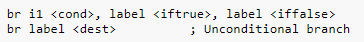
\includegraphics[height=40pt]{figures/LLVM_br_instruction_syntax.png}}}
\end{center}
\caption{\label{br_syntax}LLVM Br Instruction Syntax}
\end{figure}

Without knowing which line of instructions is forkable, generating testcases for the opposite branch is impossible. Potential forkable instructions can appear many times in a normal program, but only a few of these instructions are involved with the target symbol. If the instruction is not ``forkable,'' we have no idea if the instruction is involved with the symbol. More importantly, if an instruction cannot be forked, there is no opposite branch of that instruction. To solve this issue, I decided to use path log to guide the symbolic execution. The target binary will be run twice. The first time, a concrete input will be fed. During the execution, all of the potential forkable instructions will be logged. In my implementation, I will log four types of instruction I mention previously. For \texttt{br} instruction, instruction id and the result of \texttt{cond} will be logged. For \texttt{switch} instruction, instruction id and index of the successor will be logged. For \texttt{alloc} instruction, instruction id and allocation size will be logged. For \texttt{load} instruction, instruction id and the offset will be logged. The second run will run the program with the symbol. While exploring the path, the path log that collected during the first time can guide the execution. All the log information will be kept in a queue. If hitting the potential forkable instructions, matched the instruction id and the \texttt{cond} result/successor id/allocation size/offset with the path log in queue. If the instruction cannot be forked, the log and the execution should be the same. If it is forkable, use the log information to replace those corresponding components in the instruction. This step ensures the execution will choose the same path as the concrete input do. In \texttt{br} instruction, what will be added to constraints is based on the log. If the log is false, the negation of \texttt{cond} will be added. Otherwise, \texttt{cond} will be added. To produce the testcase that hit the other side, all we need to do is to connect the constraints (not including the newly added one) and negation of \texttt{cond} or \texttt{cond} regarding the log with the \texttt{AND} logic operator. Then we can ask solver to solve the constraints to produce a testcase that hit the opposite side. Figure \ref{testcase_generation} describes the workflow of this feature.

\begin{figure}%This [h] tells LaTeX to try to put the picture here.
                 %Without it, it will go to the top of the next page.
\begin{center}
{\mbox{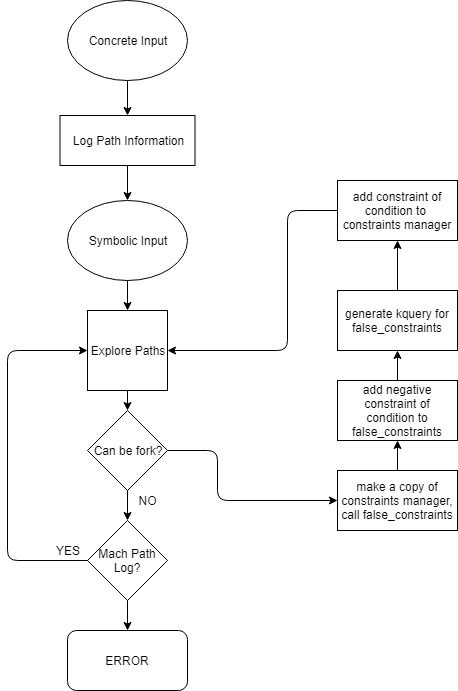
\includegraphics[height=500pt]{figures/testcase_generation.png}}}
\end{center}
\caption{\label{testcase_generation}Workflow of Generating Testcase for ``Opposite Brance''}
\end{figure}

\section{Remote Solver}

The remote solver has two part. A server that handles the HTTP request it receives and a Solver solve the queries received by a solver. Figure \ref{arch} illustrates the architecture of the remote solver. Once a \texttt{String} arrives at the Server, it will first create a file with a unique name and write the \texttt{String} it receives to the file. Then append the absolute path of that file to another file called ``Monitor'' file. This file is responsible for communicating between the server and solver. 

\begin{figure}[h]%This [h] tells LaTeX to try to put the picture here.
                 %Without it, it will go to the top of the next page.
\begin{center}
{\mbox{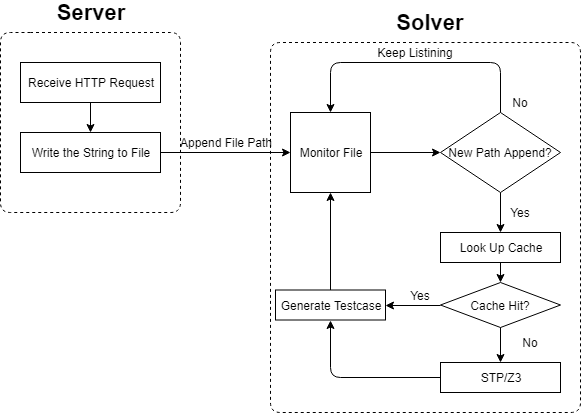
\includegraphics[height=300pt]{figures/arch.png}}}
\end{center}
\caption{\label{arch}Remote Solver Architecture}
\end{figure}

The solver is listening to ``Monitor'' file using \texttt{inotify}, which is a Linux kernel subsystem that acts to extend filesystems to notice changes to the filesystem and report those changes to applications \cite{inotify}. There are two threads in the solver. The first one is the watching module, responsible for retrieving the new appended file and push it into a thread-safe queue waiting to be solved. The other thread is the solver itself. If the queue is not empty, poping a file path once a time. Then read the content of that file, parse the content. Thanks to KLEE's implementation, they have a parse that can parse a \texttt{String} in the format of KQuery and can be used in the STP/Z3 solver directly. After parsing, the solver will check the cache map to see if there is any hit. If so, get the result from the cache map and save it as testcase. Otherwise, pass it to the solver and insert the \texttt{<constraints, result>} pair to the cache map for future use. Also, this solver will support the constraints independence optimization. 

\section{``Otherside'' Testcase Generation}
As we all know, symbolic execution is used to discover all the feasible paths of a binary, however, in some situation, we do not need to know all the paths but just some paths. To address this problem, I added a new feature to KLEE and it is called ``Otherside'' testcase generation. 

The term ``otherside" is refer to control flow direction. In the programming language level, a \texttt{if} statement may have many branches. However, in assembly level, all the ``if" statements have just two branches -- either ``True" or ``False". So, if a \texttt{br} instruction is ``True", its otherside is ``False". Otherside testcase generation aims to generate testcases that covered the otherside of the branches for a given input. Code snippet \ref{odd_or_even} shows a program that determine a number is a even number. For the given input ``2", the otherside testcase generation will generate a testcase ``1" since the this testcase will cover the otherside of the ``if" branch of the program.

\begin{spacing}{1}
{
\begin{lstlisting}[frame=shadowbox, caption={Is Even},label={odd_or_even}]
bool isEven(int n) {
    if (n % 2 == 0) {
        return True
    }
    else {
        return False
    }
}
\end{lstlisting}
}
\end{spacing}
\pagebreak
To achieve this goal, we need a concrete input for the target binary as the given input. During the execution of the given input, we need to log the path that it travels through. Then, we reset the program and make the input as symbol and use the log we collected to guide the symbolic execution.

In KLEE, instructions that will cause a ``fork'' action is the log we need to collected -- they are \texttt{br}, \texttt{switch} and \texttt{alloc}. And during the second run, we will use symbol as the input of the target binary. When it needs to fork, the path log that collected by the first run will be used to guide the execution. At the same time, the opposite condition will be concatenated to constraints using ``AND'' logic operator and send to the remote solver for testcase case generation purpose.

After two runs, we will have testcase that can hit all the opposite branches of the original concrete example.
\chapter{EXPERIMENTAL EVALUATION}%Titles must be capitalized.

In this chapter, the evaluation of the implementation will be provided. There are total three parts of the evaluation. First, exploration time for an application with the asynchronous mode comparing to synchronous mode. Second, the number of counterexamples generate by solver with the shared-cache solver. Third, with the help of the shared-cache solver, the time reduce for analysis the some applications using DFS (depth-fist-search) strategy.

\section{Exploration Time}

In this section, I will compare the exploration time for some application from GNU \texttt{COREUTILS}. KLEE will explore 20,000 paths for that application. If the application does not have 20,000 paths, then find all the feasible paths for the application. Each of the application will be run ten times. Table \ref{result_compare} shows the result of this experiment. This experiment is running on an Amazon Web Service's \texttt{t2.xlarge} machine, with four virtual CPUs and 16 gigabytes of RAM. The CPU's clock speed is up to 3.0 GHz. 

Snippet \ref{symbolic_arguments} is the symbolic arguments using for KLEE in this experiment \cite{Cadar:2008:KUA:1855741.1855756}. \texttt{posix-runtime} was enabled for making the command line arguments of the target binary symbolic.

\begin{spacing}{1}
{
\begin{lstlisting}[frame=shadowbox, caption={Symbolic Arguments},label={symbolic_arguments}]
--posix-runtime
--libc=uclibc
--search=dfs
--sym-args 0 1 10
--sym-args 0 2 2
--sym-files 1 8
--sym-stdin 8
--sym-stdout
\end{lstlisting}
}
\end{spacing}

\begin{table}[ht]
\centering
\begin{tabular}{|c|cccc|c|} 
\hline
Application               & \multicolumn{1}{c|}{Mode} & \multicolumn{1}{c|}{Average} & \multicolumn{1}{c|}{Max} & Min      & Reduce                    \\ 
\hline
\multirow{2}{*}{test ([)}        & Async                     & 233.36                       & 337.32                   & 173.26   & \multirow{2}{*}{21.92\%}  \\
                          & Sync                      & 298.88                       & 394.55                   & 253.24   &                           \\ 
\hline
\multirow{2}{*}{basename} & Async                     & 83.60                        & 84.71                    & 82.78    & \multirow{2}{*}{75.61\%}  \\
                          & Sync                      & 342.73                       & 344.42                   & 340.14   &                           \\ 
\hline
\multirow{2}{*}{chmod}    & Async                     & 230.31                       & 242.91                   & 225.66    & \multirow{2}{*}{62.30\%}  \\
                          & Sync                      & 610.96                       & 614.24                   & 607.92   &                           \\ 
\hline
\multirow{2}{*}{arch}     & Async                     & 1382.86                      & 1392.90                  & 1373.03  & \multirow{2}{*}{63.59\%}  \\
                          & Sync                      & 3797.66                      & 3901.401                 & 3753.34  &                           \\ 
\hline
\multirow{2}{*}{chgrp}    & Async                     & 243.45                       & 248.22                   & 237.51   & \multirow{2}{*}{61.75\%}  \\
                          & Sync                      & 636.55                       & 640.208                  & 633.094  &                           \\ 
\hline
\multirow{2}{*}{ls}       & Async                     & 1913.09                      & 1943.21                  & 1879.83  & \multirow{2}{*}{20.50\%}  \\
                          & Sync                      & 2406.32                      & 2409.52                  & 2403.307 &                           \\
\hline
\end{tabular}
\caption{Result of Comparing Async and Sync (unit: second)}
\label{result_compare}
\end{table}

In this experiment, it is evident that the asynchronous mode can improve the path exploration time significantly. The average time for \texttt{[} was reduced from 298.88 seconds to 233.36 seconds. It shortened the exploration by 21.92\%. For \texttt{basename} and \texttt{chmod}, the average exploration time is shortened by 75.61\% and 63.59\% respectively. \texttt{chgrp} was improved 61.75\%, and \texttt{ls} was enhanced 20.50\%

In conclusion, original KLEE spend most of its time on I/O, writing the testcases to hard drive, and waiting. With the help of the asynchronous mode, the exploration time can be shortened. The \textbf{Hypothesis 1} holds.

\section{PoC of Share-Cache Solver}

The prove of concept of the Share-Cache Solver runs in the following settings. The target binary is from GNU \texttt{Coreutils} package. The symbolic arguments remain the same as the previous experiment. Each of the application will be run twice. The solver will be terminated (cache clear) for every program. The purpose of the first run of each binary is ``building cache map.'' The second run of each binary is checking if the solver use caches to generate testcases. The solver will not be terminated between the first and second run of the same binary. The result of this experiment is shown in Table \ref{poc_table}.

\begin{table}[ht]
\centering
\begin{tabular}{|c|c|c|} 
\hline
Application & CEx Generated (1st run) & CEx Generated (2nd run)  \\ 
\hline
test ([)           & 517        & 0                                     \\ 
\hline
arch        & 294        & 0                                     \\ 
\hline
chgrp       & 190        & 0                                     \\ 
\hline
chmod       & 285        & 0                                     \\ 
\hline
chcon       & 189        & 0                                     \\ 
\hline
base64      & 133        & 0                                     \\ 
\hline
basename    & 300        & 0                                     \\
\hline
\end{tabular}
\caption{Number of Counter Examples Generated}
\label{poc_table}
\end{table}

As shown in the result, the second run will not generate any counterexamples because the first run has already built the cache. All the queries sent during the second run are exactly the same as the first run. Therefore, there is no cache missed during the second run. In other words, two runs of each program shared cache with each other. The experiment also indicates that solver the cache can help reduce the workload of the solver, and cache can be used in two different runs.

\section{Share-cache Solver Analyzing Binary}
In this section, I will use the asynchronous KLEE to analyze some binaries in GNU \texttt{Coreutils} package. First, I will run each binary for one time to collect the number of counterexamples generated as well as the solving and cache lookup time. The Share-cache solver will be terminated between each run. Then I will run those applications together. At this time, the Share-cache solver will not be terminated. The purpose of this experiment is to check if the cache can be used between different program. The target binaries are \texttt{[}, \texttt{arch}, \texttt{base64}, \texttt{basename}, \texttt{chcon}, \texttt{chgrp}, and \texttt{chmod}. 

These binaries will be executed in the following order: 1. \texttt{[} 2. \texttt{arch} 3. \texttt{basename} 4. \texttt{base64} 5. \texttt{chcon} 6. \texttt{chgrp} 7. \texttt{chmod}

Table \ref{single_run} shows the solving time, cache lookup time and number of counterexamples generated during single execution. Table \ref{combine_run} shows the result of analyzing the target binaries without terminating the shared-cache solver.

\begin{table}[ht]
\centering
\begin{tabular}{cccccc}
\hline
\multicolumn{1}{|c|}{Application} & \multicolumn{1}{c|}{Queries} & \multicolumn{1}{c|}{Caching Time} & \multicolumn{1}{c|}{Solving Time} & \multicolumn{1}{c|}{Overall Time} & \multicolumn{1}{c|}{Num. Cex} \\
\hline
\multicolumn{1}{|c|}{{test ([)}}      & \multicolumn{1}{c|}{1788}  & \multicolumn{1}{c|}{2.87}   & \multicolumn{1}{c|}{10.19} & \multicolumn{1}{c|}{13.06}  & \multicolumn{1}{c|}{517} \\ \hline
\multicolumn{1}{|c|}{arch}     & \multicolumn{1}{c|}{20000} & \multicolumn{1}{c|}{971.27} & \multicolumn{1}{c|}{0.88}  & \multicolumn{1}{c|}{972.15} & \multicolumn{1}{c|}{294} \\ \hline
\multicolumn{1}{|c|}{base64}   & \multicolumn{1}{c|}{20000} & \multicolumn{1}{c|}{42.38}  & \multicolumn{1}{c|}{1.08}  & \multicolumn{1}{c|}{43.46}  & \multicolumn{1}{c|}{133} \\ \hline
\multicolumn{1}{|c|}{basename} & \multicolumn{1}{c|}{14071} & \multicolumn{1}{c|}{3.38}   & \multicolumn{1}{c|}{0.56}  & \multicolumn{1}{c|}{3.94}   & \multicolumn{1}{c|}{300} \\ \hline
\multicolumn{1}{|c|}{chcon}    & \multicolumn{1}{c|}{20000} & \multicolumn{1}{c|}{11.42}  & \multicolumn{1}{c|}{1.00}  & \multicolumn{1}{c|}{12.42}  & \multicolumn{1}{c|}{189} \\ \hline
\multicolumn{1}{|c|}{chgrp}    & \multicolumn{1}{c|}{20000} & \multicolumn{1}{c|}{14.74}  & \multicolumn{1}{c|}{1.61}  & \multicolumn{1}{c|}{16.35}  & \multicolumn{1}{c|}{190} \\ \hline
\multicolumn{1}{|c|}{chmod}    & \multicolumn{1}{c|}{20000} & \multicolumn{1}{c|}{10.91}  & \multicolumn{1}{c|}{1.07}  & \multicolumn{1}{c|}{11.98}  & \multicolumn{1}{c|}{285} \\ \hline
Total                          &                            & 1056.97                 & 16.40                  & 1073.36                 & 1908                    
\end{tabular}
\caption{Caching and Solving Time For Analyzing a Single Binary (unit: second)}
\label{single_run}

\vspace{2cm}

\begin{tabular}{cccccc}
\hline
\multicolumn{1}{|c|}{Application} & \multicolumn{1}{c|}{Queries} & \multicolumn{1}{c|}{Caching Time} & \multicolumn{1}{c|}{Solving Time} & \multicolumn{1}{c|}{Overall Time} & \multicolumn{1}{c|}{Num. Cex} \\ \hline
\multicolumn{1}{|c|}{{test ([)}}      & \multicolumn{1}{c|}{1788}  & \multicolumn{1}{c|}{2.88}    & \multicolumn{1}{c|}{10.23} & \multicolumn{1}{c|}{13.11}   & \multicolumn{1}{c|}{518} \\ \hline
\multicolumn{1}{|c|}{arch}     & \multicolumn{1}{c|}{20000} & \multicolumn{1}{c|}{3189.86} & \multicolumn{1}{c|}{0.43}  & \multicolumn{1}{c|}{3190.29} & \multicolumn{1}{c|}{75}  \\ \hline
\multicolumn{1}{|c|}{basename} & \multicolumn{1}{c|}{14071} & \multicolumn{1}{c|}{6.71}    & \multicolumn{1}{c|}{0.23}  & \multicolumn{1}{c|}{6.94}    & \multicolumn{1}{c|}{98}  \\ \hline
\multicolumn{1}{|c|}{base64}   & \multicolumn{1}{c|}{20000} & \multicolumn{1}{c|}{38.77}   & \multicolumn{1}{c|}{0.77}  & \multicolumn{1}{c|}{39.54}   & \multicolumn{1}{c|}{71}  \\ \hline
\multicolumn{1}{|c|}{chcon}    & \multicolumn{1}{c|}{20000} & \multicolumn{1}{c|}{9.11}    & \multicolumn{1}{c|}{0.05}  & \multicolumn{1}{c|}{9.16}    & \multicolumn{1}{c|}{98}  \\ \hline
\multicolumn{1}{|c|}{chgrp}    & \multicolumn{1}{c|}{20000} & \multicolumn{1}{c|}{16.75}   & \multicolumn{1}{c|}{0.22}  & \multicolumn{1}{c|}{16.97}   & \multicolumn{1}{c|}{50}  \\ \hline
\multicolumn{1}{|c|}{chmod}    & \multicolumn{1}{c|}{20000} & \multicolumn{1}{c|}{9.21}    & \multicolumn{1}{c|}{0.05}  & \multicolumn{1}{c|}{9.26}    & \multicolumn{1}{c|}{86}  \\ \hline
Total                          &                            & 3273.28                      & 11.98                      & 3285.26                      & 996
\end{tabular}
\caption{Caching and Solving Time For Analyzing 7 Binaries (unit: second)}
\label{combine_run}
\end{table}

Without the cross-binary cache share solver, the total number of testcases generated by the solver is 1,908 for analyzing all these seven target binaries. With the cross-binary cache share solver, this number reduced from 1,908 to 996. That's a 47.83\% reduction. With such reduction in the number of counterexamples generated by the solver, the solving time (time that spend in STP/Z3 solver) dropped from 16.40 seconds to 11.98 seconds. The cross-binary shared-cache solver spends 26.95\% less time in STP/Z3.

Cache lookup time get hurts from the increase of cache map size because of the cache look up mechanism. The solver follows the following cache lookup policy. First, check if the expression exists in the cache map. If yes, then it is a direct cache hit. If not, iterate through the cache map, try all of the answers to see if any of these solutions fit the expression. If yes, then it is an indirect cache hit. Otherwise, it is a cache miss. The worst case of time complexity for the strategy of cache look up is $O(n)$ since the solver needs to iterate through the whole map to see if there is any answer satisfies the expression if there is no direct hit. Due to the increase of cache size, the cache map size will go up. As we can see, these binaries more or less have indirect hits, therefore the cache look up takes longer. 

If the remote solver does not allow the indirect cache hit, the number of counterexample will increase a lot. Take the example of \texttt{arch}, the time for solving indirect hits using STP/Z3 takes longer than the current situation (first 7000 testcase spends around 1500 seconds in STP/Z3, about 21 second in cache lookup). So there is a trade off here. Allowing indirect hits will cause increase of the cache lookup time but decrease the number of counterexamples generated. Disable indirect cache hit will cause the number of counterexamples and the time for solving those indirect hits in STP/Z3 probably takes longer.

\section{Cache Strategy Improvement}
As the result shown above, current caching strategy is not that perfect. Therefore, a new strategy has been added to the remote constraints solver, that is let the solver race with the cache lookup.

In the original implementation, once the remote constraint solver receive the kquery, it will start lookup the cache in the cache pool. The original caching look up strategy has two steps. First check if there is a direct cache hit. Second, if there is no direct cache hit,try all the result in cache pool to see if any result meets the constraints. Therefore, the worst situation for cache lookup is $O(n)$. With more and more cache gets into the cache pool, this time will increase.

Moreover, in reality, some cache lookup time will slower than solve the constraints directly. Therefore, in this improved cache lookup strategy, the remote solver have multithreads. One of them is responsible for cache lookup, and the other one is responsible for solve the query directly. And the solver will return the result whoever comes back first. 

When testing the \texttt{gnu util} package, the average time form solving a query is 0.01 seconds, and the average time for solving query directly is 0.002 second. Under this strategy, the expensive ``indirect cache`` strategy is abandoned since solving the query is much faster than finding a indirect cache hit. 
\chapter{SUMMARY AND CONCLUSION}%Titles must be capitalized.

\section{Summary}
In this research, an asynchronous KLEE was implemented also a remote solver was built to work with the asynchronous mode. Compare to the original KLEE, the major difference of the asynchronous KLEE is that it has an asynchronous solver. Previously, when an \texttt{ExecutionState} was terminated, it will trigger a function called \texttt{ProcessTestcase}. In this function, KLEE will extract the constraints from the \texttt{ExecutionState}, parse it to a data structure that can use the interface that provided by STP/Z3 solver. Then KLEE will wait for solver's response. After receiving the result from solver, KLEE will wrapped up the answer and write the testcase to disk. What asynchronous KLEE does in \texttt{ProcessTestcase} is, it extracts the constraints from the \texttt{ExecutionState}, converted to a \texttt{String} in KQuery format, which is a textual representation of constraints. Instead of sitting tight and waiting for solver's response, the asynchronous KLEE sends out a string of query command using HTTP \texttt{POST} method to a remote solver. After sending the query out, the asynchronous KLEE immediately start to execute next \texttt{ExecutionState} in its \texttt{ExecutionState} pool. 

The asynchronous KLEE optimize the procedure in producing testcase for a \texttt{ExecutionState}. In the original KLEE, it wastes a lot of time in generating testcases. Through the experiment in chapter 4, it has already been proved that the asynchronous KLEE can shorten the time for exploring paths significantly when comparing to the original version of KLEE.

A remote solver was also been wrapped up to serve the asynchronous KLEE. There are two parts of the remote solver, the HTTP server and an STP/Z3 solver. The HTTP solver is responsible for receiving query command \texttt{String} from asynchronous KLEE. Then, the server will create a file and write the query command it just receives to that file. Also, the absolute path of that file will be appended to a file called ``monitor file.'' It performs like a queue because the solver is watching the change of this file using Linux kernel subsystem called \texttt{inotify}. Once a new path was appended, the solver will know a query command just came in and is waiting for the result.

The solver's responsibility is solving constraints and producing testcases. When there is a path appended to the ``monitor file,'' the solver will read the contents of that file and parse the file to a data structure that can communicate with STP/Z3 solver. Here, some optimization will be performed before the query gets into the STP/Z3 solver. First of all, the query will be chopped into small pieces. Those pieces are independents, in another word, those small pieces is also a valid expression. This step was called ``independence constraints.'' Second, the solver will check if the expressions have been solved previously. To accomplish this goal, the solver will save a cache map in RAM. The key of the cache map is the expression, and value is the answer. If the answer exists, the expression will not be passed into the STP/Z3 solver. Otherwise, the \texttt{expression, answer} pair will be inserted into the cache map after STP/Z3 solves the expression. Unlike KLEE's implementation, the solver keeps alive until the user terminates it. Therefore, sharing cache cross binary is possible. In KLEE's implementation, the solver instance will be terminated when execution completed and the cache will be deleted. If we use KLEE to analyze the same application, it still needs to solve the expression instead of pulling out the answer directly from the cache. This situation does not happen in the remote solver. Not only the same binary can share cache, but also another program since the remote solver does not know which program is being analyzed. All it knows are just expressions. Once the there is a same expression in the cache, it will pull out the answer from the cache instead of solving it. The experiment in Chapter 4 has proved that the solver share caches cross binaries.

\section{Future Work}
Although the asynchronous KLEE has some advantages on shortening the exploration time on the engine side as well as save some extra work on the solver side, it still has many places to work on in the future. Using cache in the solver is a perfect idea, but how to save the cache can be optimized a little bit more. In the current implementation, the cache map is saved in RAM. The access time of the RAM is fast. However, when the solver keeps working, the size of the cache map is growing. Ultimately, the machine will probably run out of memory. Also, if the solver died accidentally, such as having power outage issue, the cache will be unrecoverable. To address these problems, the cache should be stored in another place. For example, in a file or in a database. And this kind of action will sacrifice the access time. 

% \begin{appendices}
% 	\input{extended_results}
% \end{appendices}

\newpage
\bibliographystyle{plainnat}
\bibliography{dissertation}

\end{document}
